\documentclass[mythesis.tex]{subfiles}
\begin{document}
% tells latex when compiling a subfile what chapter number this document is
% set the chapter to minus one as \chapter will increment the counter
\setcounter{chapter}{3}
\chapter{Model of the Physical Deuteron}

All of the basic conceptual machinery is now in place to extend the simple
scalar model calculations to the more realistic case of spin-$\frac{1}{2}$,
isospin-$\frac{1}{2}$
nucleons interacting through the exchange of a variety of mesons
with various masses, spins, parities and isospins. All quantities can be
calculated
just as in the scalar case, but the calculations are complicated considerably
by the necessity of dealing with relativistic particles with spin. The
spin-$\frac{1}{2}$ nucleons are now defined by propagators which are
four-dimensional matrices in the Dirac-spinor space and couplings of mesons
to the nucleons are in general represented by operators in the Dirac-space
and operators in the isospin space of the nucleons. Therefore, many of the
quantities which are simply represented by numbers in the scalar model
will be matrices or tensors in the realistic model. While tedious, these
complications can be dealt with in relatively straight forward ways by
constructing coupled integral equations projected onto suitable subspaces.
It is useful to examine some of the quantities which contribute to the
realistic calculation in order to understand how to extend the previous
discussion to cover the more realistic model.

The Bethe-Salpeter vertex function for the spin-1 deuteron can be written
as
%
\begin{equation}
\left( \Gamma(p,P)\cdot \xi_{\lambda_d}(P) {\cal C}\right)_{ab}
\end{equation}
where $\xi_{\lambda_d}(P)$ is the polarization four-vector for the deuteron,
$\cal C$ is the Dirac charge conjugation matrix ,
the subscripts $a$ and $b$ are indices in the Dirac spinor space, and
$\Gamma^\mu$ can be determined by basic symmetry arguments to have the
general form:
\begin{eqnarray}
%
\Gamma^\mu(p,P)&=&f_1(p^2,p\cdot P)\gamma^\mu
+ g_1(p^2,p\cdot P)\frac{p^\mu}{m}\nonumber\\
& &+\frac{\not{\!p}_2-m}{m}\left( f_2(p^2,p\cdot P)\gamma^\mu
+g_2(p^2,p\cdot P)\frac{p^\mu}{m}\right)\nonumber\\
& &+\left( f_2(p^2,-p\cdot P)\gamma^\mu
+g_2(p^2,-p\cdot P)\frac{p^\mu}{m}\right) \frac{\not{\!p}_1+m}{m}\nonumber\\
& &+\frac{\not{\!p}_2-m}{m}\left( f_4(p^2,p\cdot P)\gamma^\mu
+g_4(p^2,p\cdot P)\frac{p^\mu}{m}\right) \frac{\not{\!p}_1+m}{m}
\end{eqnarray}
%
where $p_1=\frac{P}{2}+p$ and  $p_2=\frac{P}{2}-p$.
This satisfies the generalized Pauli symmetry requiring that
%
\begin{equation}
\Gamma^\mu(p,P)=-{\cal C}\Gamma^{\mu T}(-p,P){\cal C}^{-1}.
\end{equation}
%
Note that for given values of $p$ and $P$, the vertex function depends upon
eight scalar functions, two pairs of which are related by inversion of $p$.
In the case of the constrained spectator vertex function where particle 1
is on its positive energy mass shell, only four of these functions
contribute. Therefore, the general Bethe-Salpeter vertex and wave functions
can be represented by eight radial wave functions while the spectator
constrained vertices and wave functions have only four radial wave
functions.

The single-nucleon current operator to be used with factorable interaction
vertices is given by \cite{GrossandRiska}:
%
\begin{eqnarray}
\vspace{12pt}
J^{(i)\mu} (p',p) &= &F_1(Q^2) f_0(p'^2,p^2) \,  \gamma^\mu +
\frac{F_2(Q^2)}{2m} h_0(p'^2,p^2) \, i \sigma^{\mu \nu}
q_\nu \nonumber\\
& & + F_3(Q^2) g_0(p'^2,p^2) \,  \frac{\not{\!p}'-m}{2m} \,  \gamma^\mu  \,
 \frac{\not{\!p}-m}{2m} \label{offshellcur}
\end{eqnarray}
%
where
%
\begin{equation}
f_0(p'^2,p^2) \equiv \frac{h(p^2)}{h(p'^2)} \,  \frac{m^2-p'^2}{p^2-p'^2}+
\frac{h(p'^2)}{h(p^2)}  \, \frac{m^2-p^2}{p'^2-p^2},
\end{equation}
%
\begin{equation}
g_0(p'^2,p^2) \equiv \left( \frac{h(p^2)}{h(p'^2)}-\frac{h(p'^2)}{h(p^2)}
\right) \frac{4m^2}{p'^2-p^2}
\end{equation}
%
and $h_0(p'^2,p^2)$ is an arbitrary function subject only to the constraint
that $h_0(m^2,m^2)=1$. In the calculations presented here, this function is
chosen to be $h_0(p'^2,p^2)=f_0(p'^2,p^2)$, for simplicity.

By invoking Lorentz invariance, current conservation and parity, the
general form of the elastic electromagnetic current matrix element for
elastic electron scattering from the deuteron can be shown to have the
general form \cite{ACG}:
%
\begin{eqnarray}
{\cal J}^\mu_{\lambda_d' \lambda_d} (P',P) & = & - \biggl \{ G_1 (Q^2)
(\xi^*_{\lambda_d'}(P') \cdot \xi_{\lambda_d}(P) )
(P' + P)^\mu \nonumber \\
& + & G_2 (Q^2) \Bigl [ \xi^\mu_{\lambda_d}(P)
(\xi^*_{\lambda_d'}(P') \cdot q ) -
\xi^{\mu *}_{\lambda_d'}(P') (\xi_{\lambda_d}(P) \cdot q)
\Bigr ] \nonumber \\
& - & G_3 (Q^2) {1 \over 2 M_d^2} (\xi^*_{\lambda_d'}(P')
\cdot q ) ( \xi_{\lambda_d}(P) \cdot q) (P' + P) ^\mu
\biggr \}
\end{eqnarray}
%
The $G_i$'s are related to the charge, magnetic and quadrupole form factors
by:
%
\begin{eqnarray}
G_C & = & G_1 + {2 \over 3} \eta G_Q \nonumber\\
G_M & = & G_2  \nonumber\\
G_Q & = & G_1 - G_2 + (1 + \eta) G_3
\end{eqnarray}
%
where
%
\begin{equation}
\eta=\frac{Q^2}{4 M_d^2}
\end{equation}

The cross section for elastic electron-deuteron scattering is:
\begin{equation}
{d \sigma \over d \Omega} = \left( {d \sigma \over d \Omega}
\right)_{Mott}\frac{1}{ 1 + \frac{2 E }{ M_d} \sin^2
(\theta / 2)  } \left [ A (Q^2) + B (Q^2) \tan^2 {\theta \over 2}
\right ]
\end{equation}
%
where the structure functions $A(Q^2)$ and $B(Q^2)$ can be defined in terms
of the form factors $G_C$, $G_M$ and $G_Q$ as:
%
\begin{eqnarray}
A (Q^2) & \equiv & G_C^2 (Q^2) + {Q^2 \over 6 M_d^2} G_M^2 (Q^2)
+ {Q^4 \over 18 M_d^4} G_Q^2 (Q^2) \nonumber\\
B (Q^2) & \equiv & {Q^2 \over 3 M_d^2} \left ( 1 +
{Q^2 \over 4 M_d^2} \right ) G_M^2 (Q^2) \nonumber
\end{eqnarray}
%
The charge and quadrupole form factors can be separated by measuring
the tensor polarization $T_{20}$ in a polarization experiment.
This is defined as:
%
\begin{equation}
T_{20} (Q^2) = -{\sqrt 2 Q^2 \over 3 M_d^2} {G_C G_Q + (Q^2 / 12 M_d^2)
G_Q^2 \over G_C^2 + (Q^4 / 18 M_d^4) G_Q^2}
\end{equation}
and is sometimes denoted as $\tilde t_{20}$.

\begin{table}
\caption{This is a spurious table.}
\label{classes}
\begin{center}
\begin{tabular}{cccccccccc}\hline\hline

  & {$U$}  & {$T_{10}$}  & {$T_{20}$}  &
{$Im~T_{11}$}  & {$ReT_{11}$}  & {$ImT_{21}$}  &{$ReT_{21}$}  & {$ImT_{22}$}
  & {$ReT_{22}$}  \\
\hline
{$U$}    & I  & I   & I   & II  & II  & II  & II  & I   & I  \\
{$P_n$}  & I  & I   & I   & II  & II  & II  & II  & I   & I  \\
{$P_s$}  & II & II  & II  & I   & I   & I   & I   & II  & II  \\
{$P_l$}  & II & II  & II  & I   & I   & I   & I   & II  & II \\ \hline\hline
\end{tabular}
\end{center}
\end{table}

Reference \cite{FVOHB} describes in considerable detail the application
of the
spectator equation to nucleon-nucleon scattering and the deuteron bound
state. Four models are presented for the NN interaction. Each model has
been fitted to the NN phase shift data of Arndt and Roper, SP89
\cite{ArndtandRoper}  with the aid of the error
matrix obtained in the phase shift fit. These fits are constrained such
that the deuteron bound state mass is correct. The resulting phase shift
calculations are then compared to the data base and typically obtain a
$\chi^2$ per datum of approximately 2 for energies from $0~MeV$ to $225~MeV$
of laboratory kinetic energy. This is quite good for a one-boson-exchange
model.

An unusual feature of these calculations is that some care has been taken
in allowing for meson-nucleon couplings that contain off-shell couplings
which are not usually present in such models. For example, the basic form
of the $\pi NN$ coupling is chosen to be \cite{FVOHA,FVOHB,BuckandG}:
%
\begin{equation}
g_\pi \left[ \lambda_\pi \gamma^5+(1-\lambda_\pi)\frac{(\not{p}-\not{p'})}
{2m}\gamma^5\right]
\end{equation}
%
where $0\leq \lambda_\pi\leq 1$ is a parameter which extrapolates the
coupling between pseudoscalar and pseudovector coupling. This coupling is
independent of $\lambda_\pi$ when the nucleons are on mass shell, so
models with differing values of $\lambda_\pi$ differ in their off-shell
content. All meson-nucleon interactions also include factorable form factors
as in the scalar model presented above.

Two of the models from Refs. \cite{FVOHA,FVOHB} are used in the calculations of
elastic
electron-deuteron scattering that will be presented here. These models are
labelled Model IB and Model IIB. Model IB has a kernel containing four
mesons: $\pi$, $\sigma$, $\omega$ and $\rho$. The pion mixing parameter
$\lambda_\pi$ was adjusted as part of the fitting procedure and has a
value of $\lambda_\pi=0.216$. That is, there is a 22\% admixture of
pseudo-scalar pion coupling. A total of ten parameters are adjusted in
the fitting procedure. Model IIB has six mesons: $\pi$, $\eta$, $\sigma$,
$\sigma_1$, $\omega$ and $\rho$. The $\sigma_1$ meson is a scalar-isovector
companion to the $\sigma$ with a mass comparable to the $\sigma$ mass.
The pion mixing parameter was fixed at $\lambda_\pi=0$ for pure pseudovector
coupling. A total of thirteen parameters were adjusted in the fitting
procedure.

\begin{figure}
     \centerline{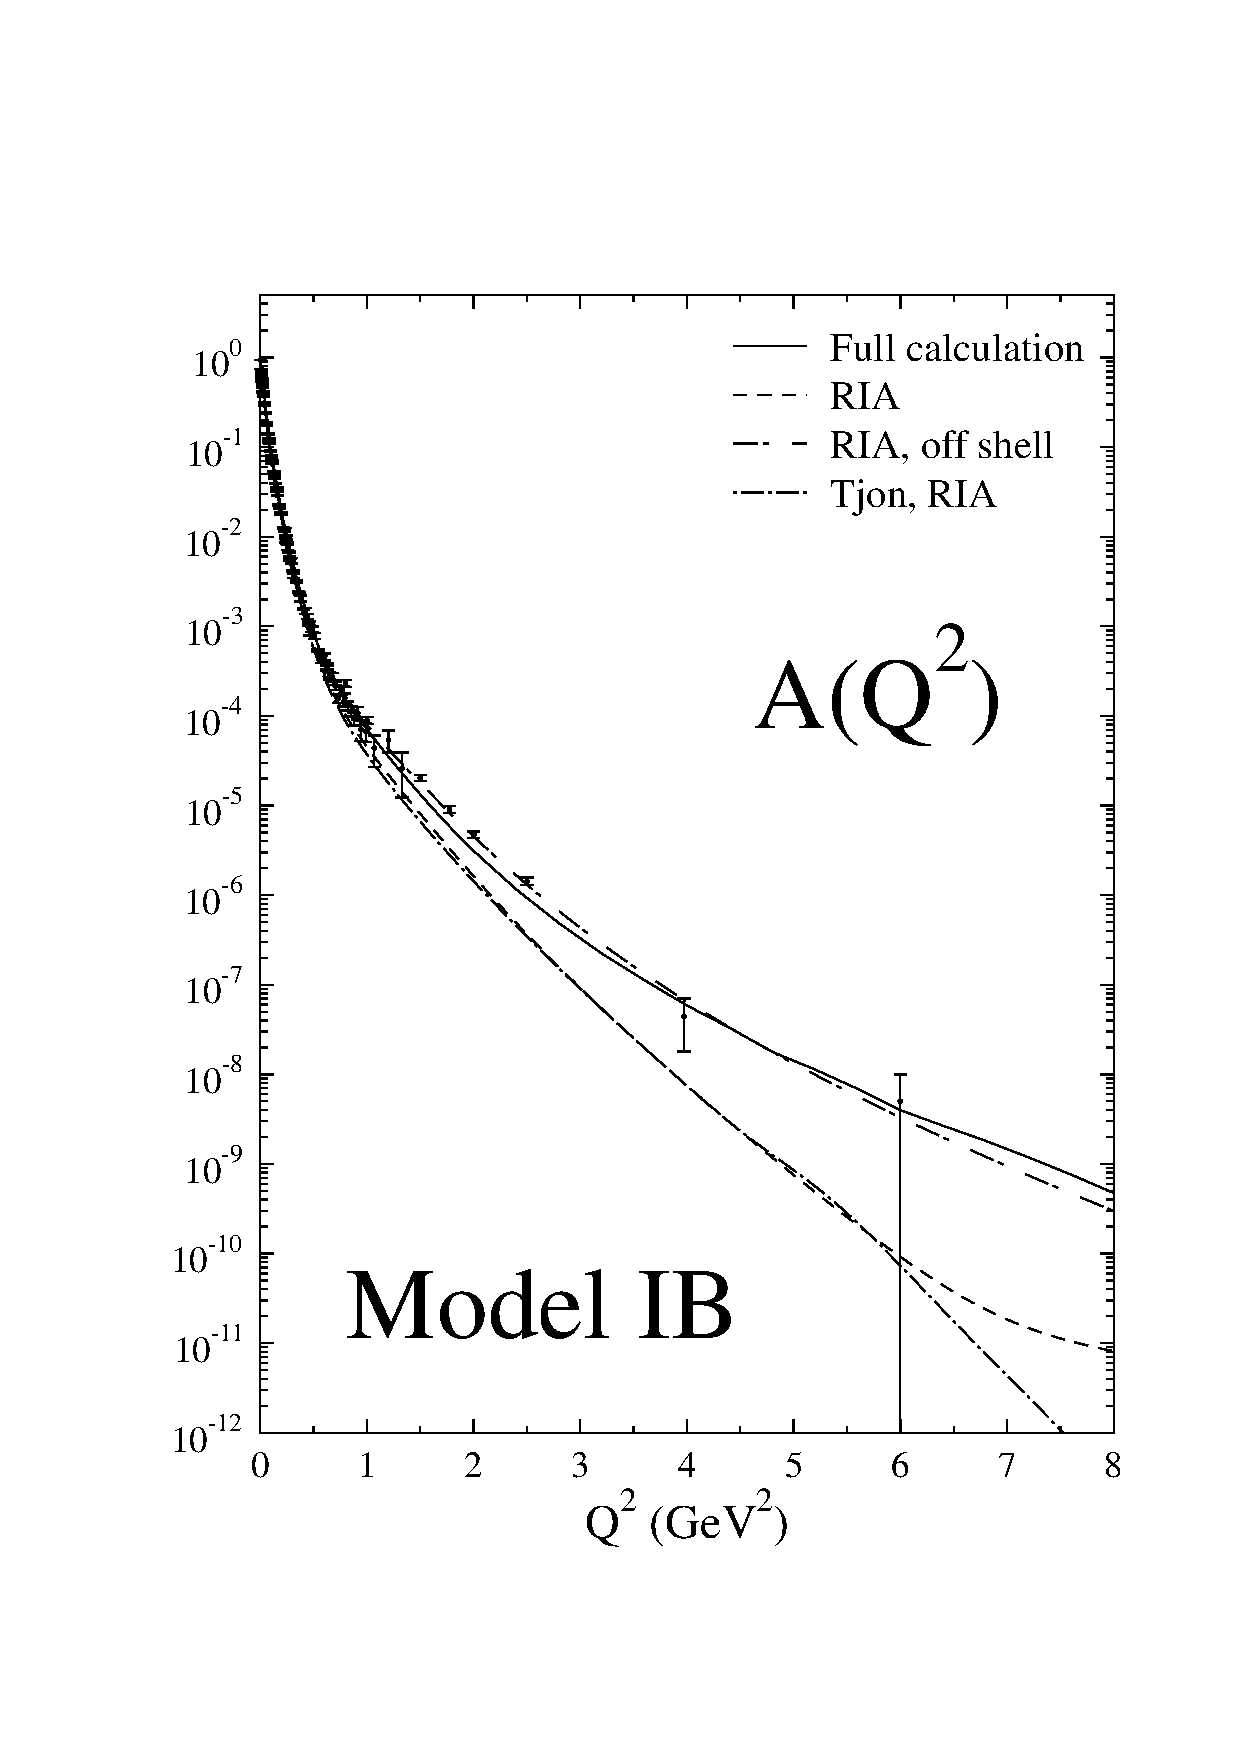
\includegraphics[width=2.75in]{graphics/a_ib.pdf}
     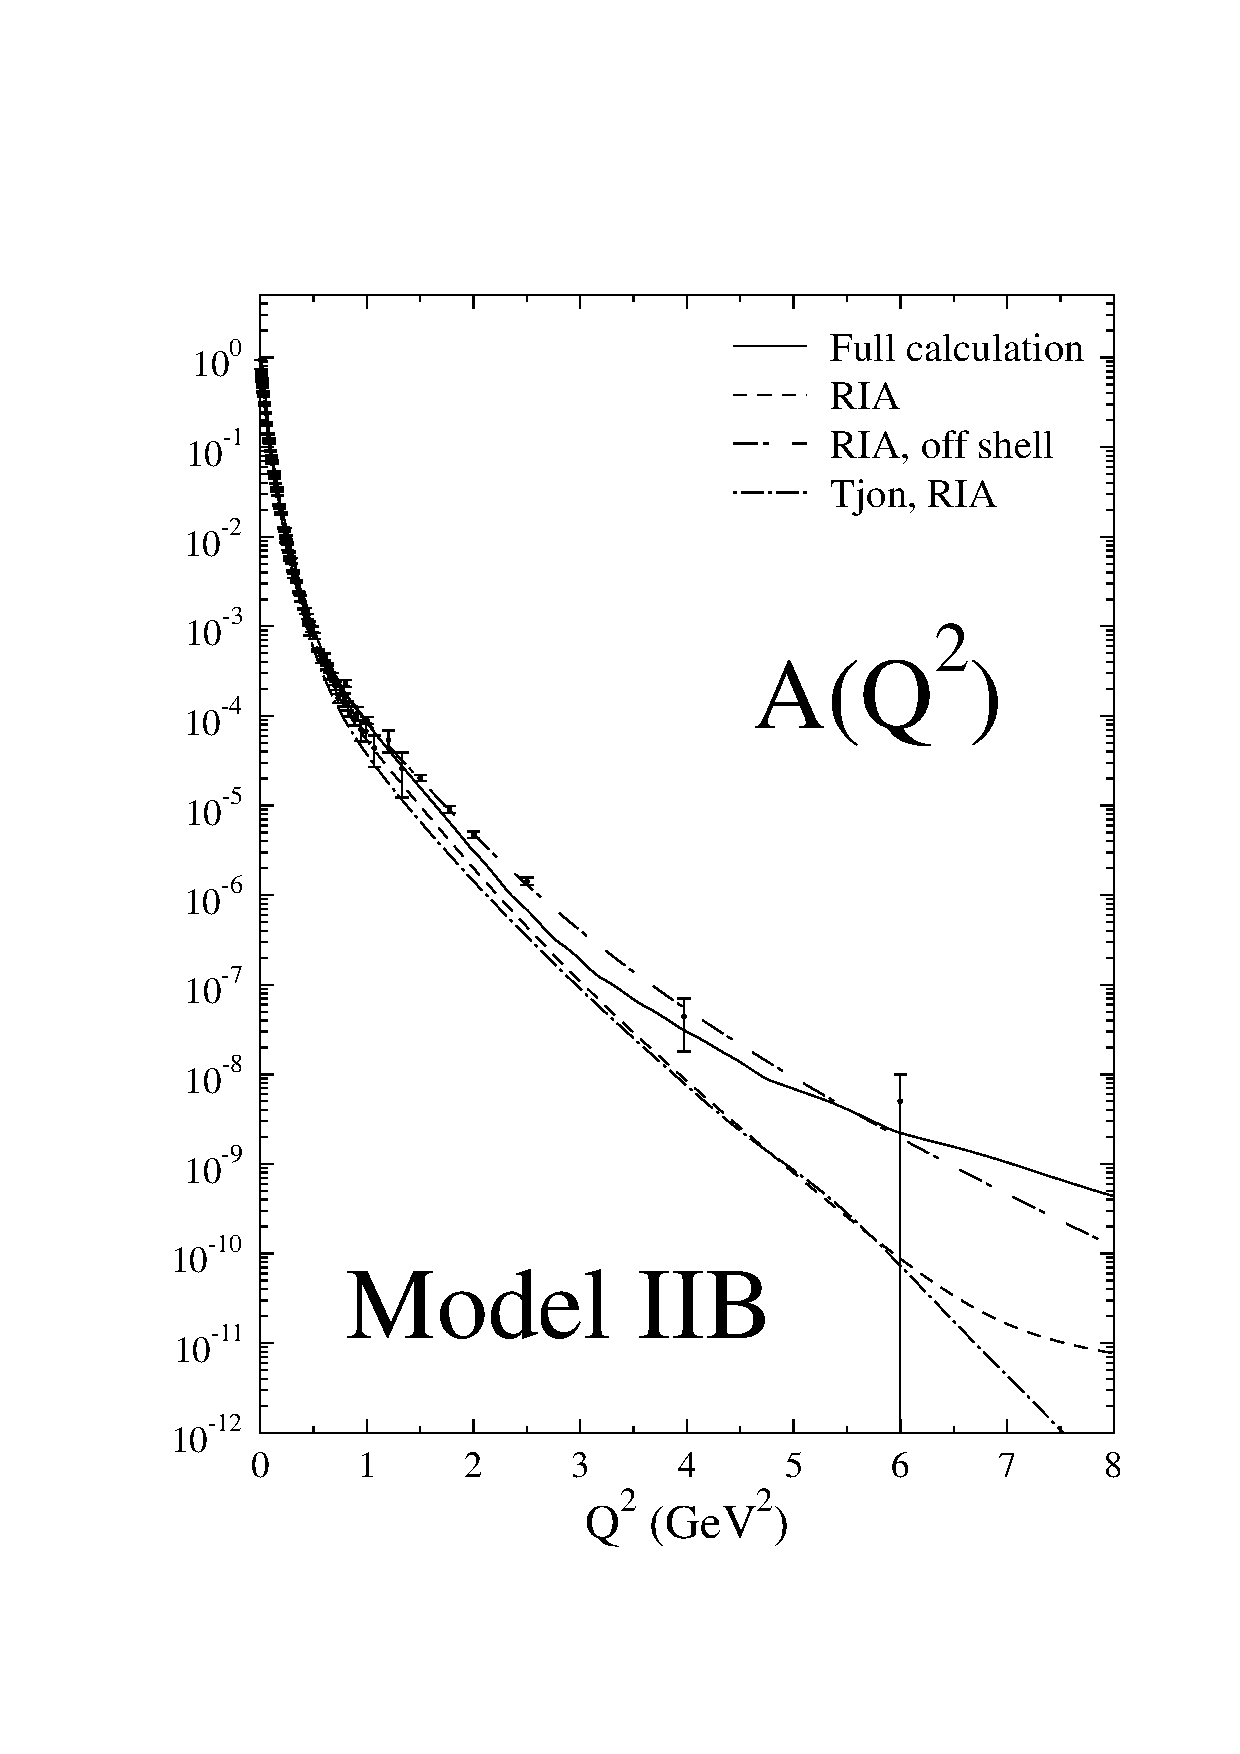
\includegraphics[width=2.75in]{graphics/a_iib.pdf}}
\vspace{-24pt}
      \centerline{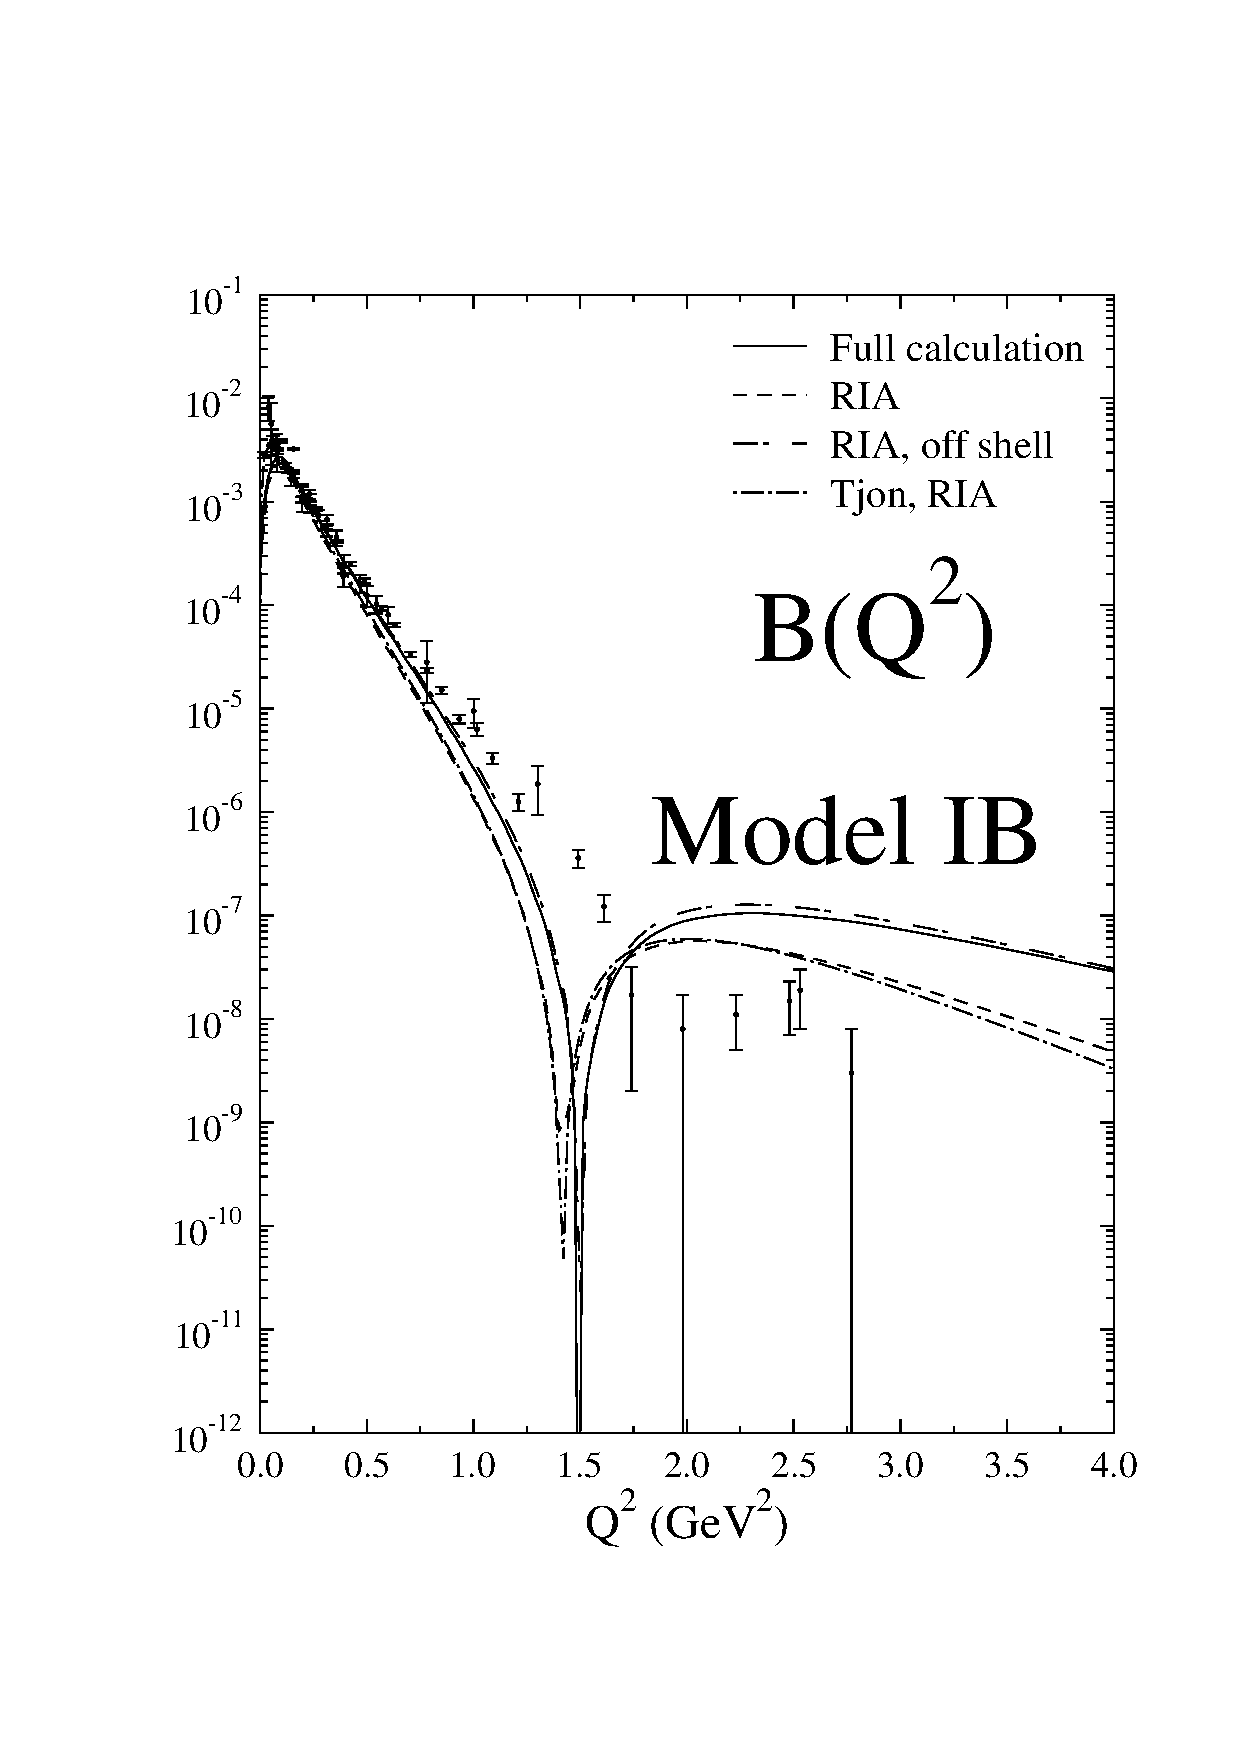
\includegraphics[width=2.75in]{graphics/b_ib.pdf}
     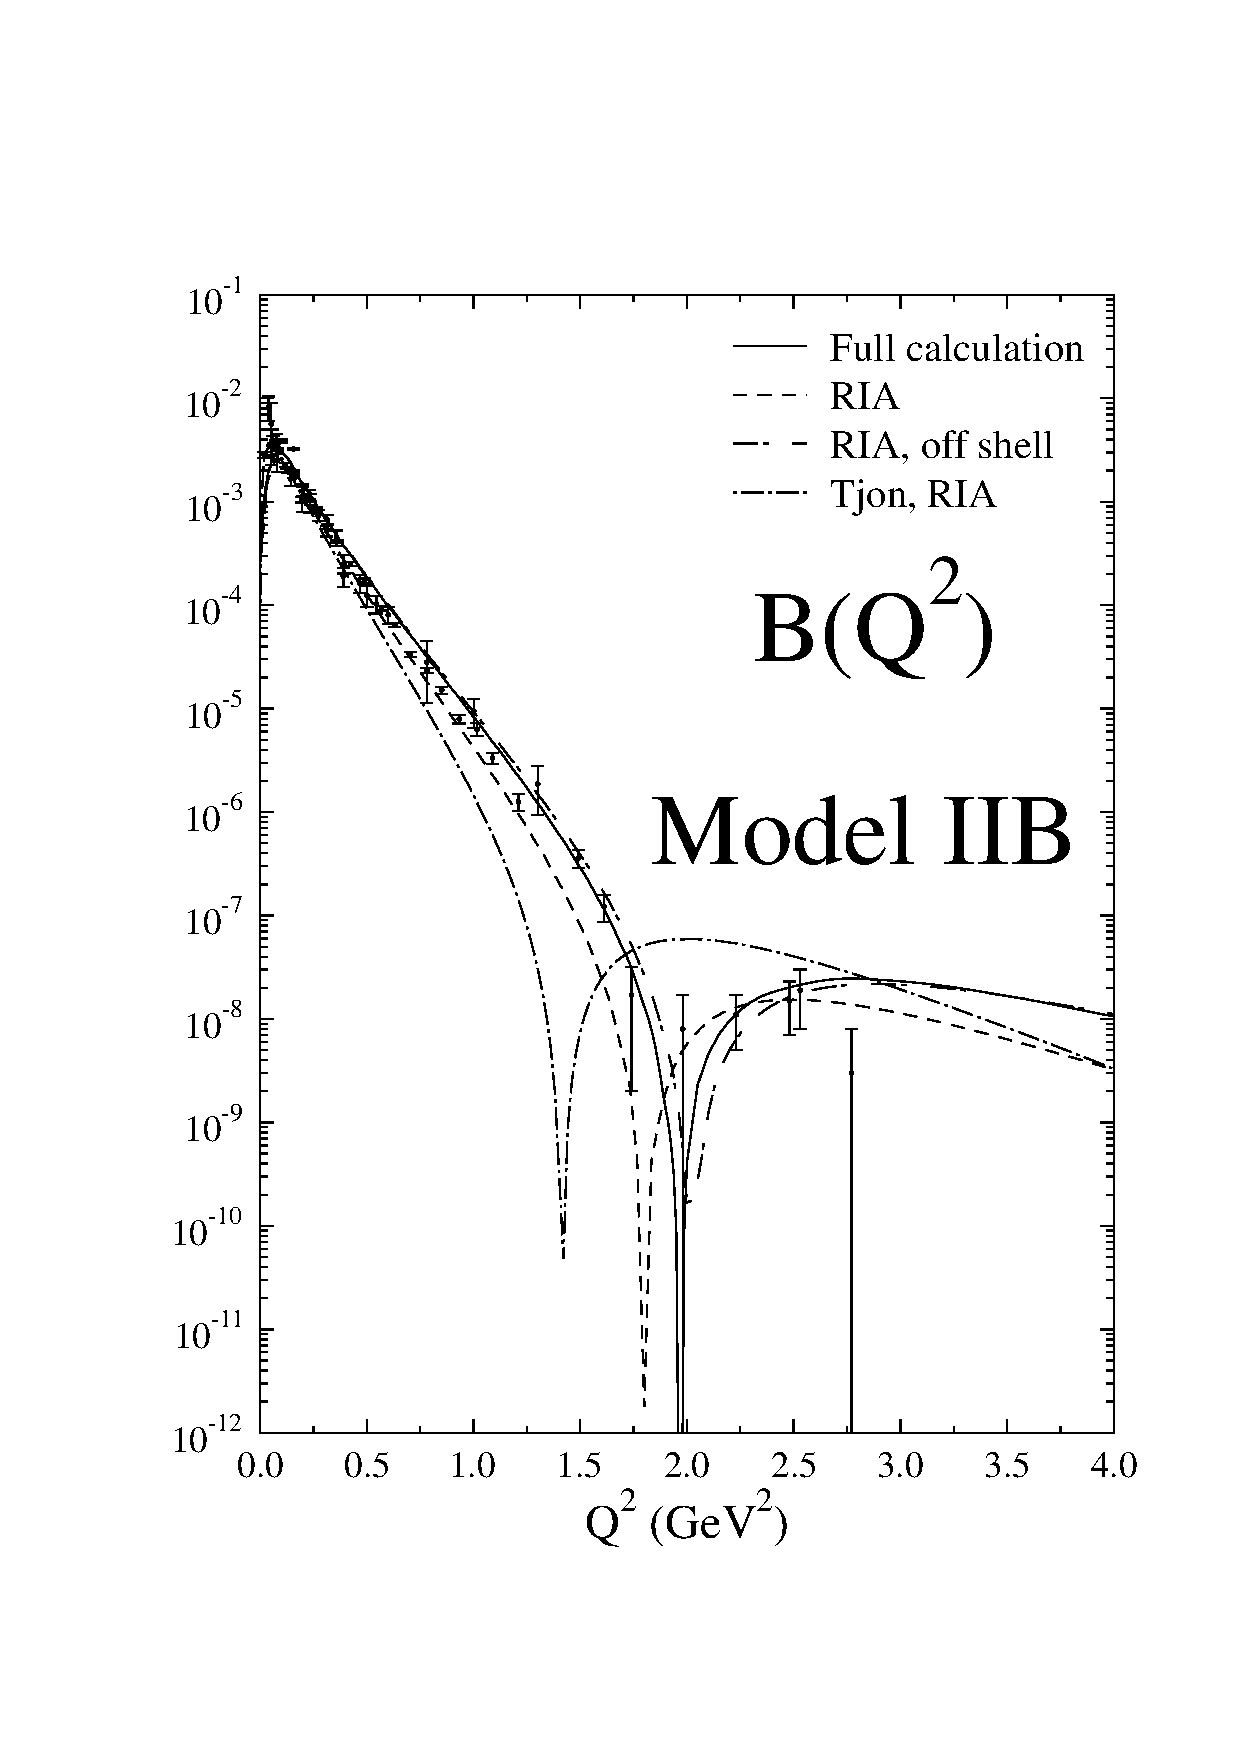
\includegraphics[width=2.75in]{graphics/b_iib.pdf}}
  \caption{$A$ and $B$ structure functions for models IB and IIB using the
           spectator equation.}\label{structure}
\end{figure}

Figure \ref{structure} shows preliminary results for the $A$ and $B$
structure functions as
calculated for models IB and IIB using the Galster form of the dipole
parameterization of the single-nucleon electromagnetic form factors
\cite{Gals71}.
Four calculations are presented for each
case. The full calculation is the result of calculating diagrams
(\ref{Gcurrent}a), (\ref{Gcurrent}b) and (\ref{Gcurrent}c). Since the
deuteron is an isoscalar, the only exchange currents as represented by
diagram (\ref{Gcurrent}d) must be isoscalar and in this case are transition
currents of the type $\rho\pi\gamma$. Such corrections are in the process
of being calculated for these models, but are not yet available. The three
remaining calculations are RIA calculations. One uses the usual on-shell
current operator which corresponds to setting $f_0=h_0=1$ and $g_0$ and is
labelled ``RIA''. The
second uses the full off-shell current described by (\ref{offshellcur}) and
is labelled ``RIA, off shell''.
The third is the Bethe-Salpeter RIA of Zuilhof and Tjon \cite{Zuilhof}
which corresponds
to diagrams (\ref{BScurrent}a) and (\ref{BScurrent}b), only the usual form
of the on-shell current operator is used. Use of the off-shell
single-nucleon current causes an increase in size for all of the structure
functions. The full calculations show little model dependence for $A(Q^2)$.
The full calculations of $A(Q^2)$ are still somewhat below the data at
intermediate $Q^2$ and will require some contribution from isoscalar
exchange currents, although less than previous calculations. $B(Q^2)$
shows substantial model dependence with the position of the diffraction
minimum moved to higher $Q^2$. Indeed, the full calculation is in remarkably
good agreement with the data.
This calculation may indeed be too good in that it leaves little room for
exchange current contributions. There is, however, some controversy as
to the strength of the isoscalar exchange currents with recent calculations
suggesting that they may, indeed, be small \cite{ItoGross}. Since models IB
and IIB are
largely equivalent on mass shell, the sensitivity of $B(Q^2)$ is likely
the result of the off-mass-shell differences of the two interactions. This
suggests that electromagnetic processes may well provide useful information
about the off-shell behavior of strong interaction models.


\begin{figure}
     \centerline{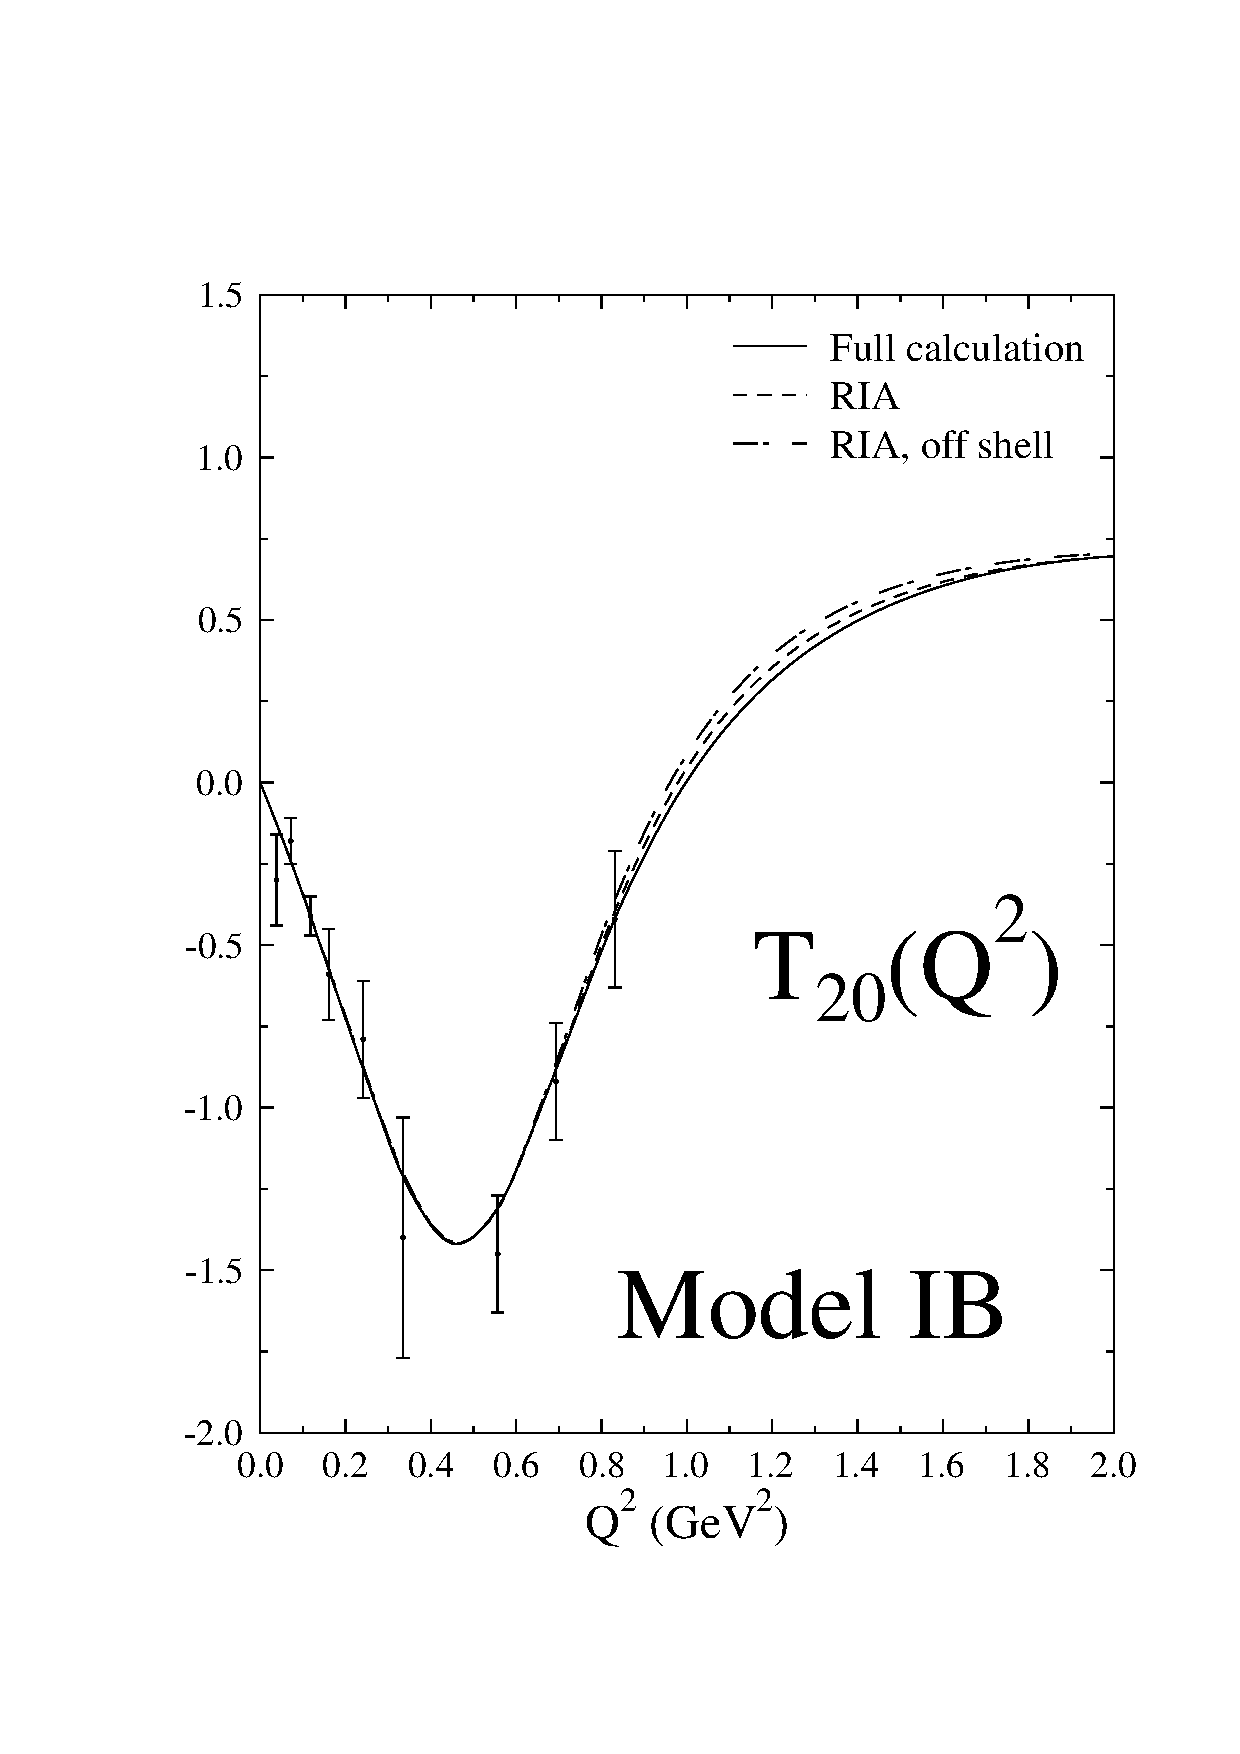
\includegraphics[width=2.75in]{graphics/t20_ib.pdf}
     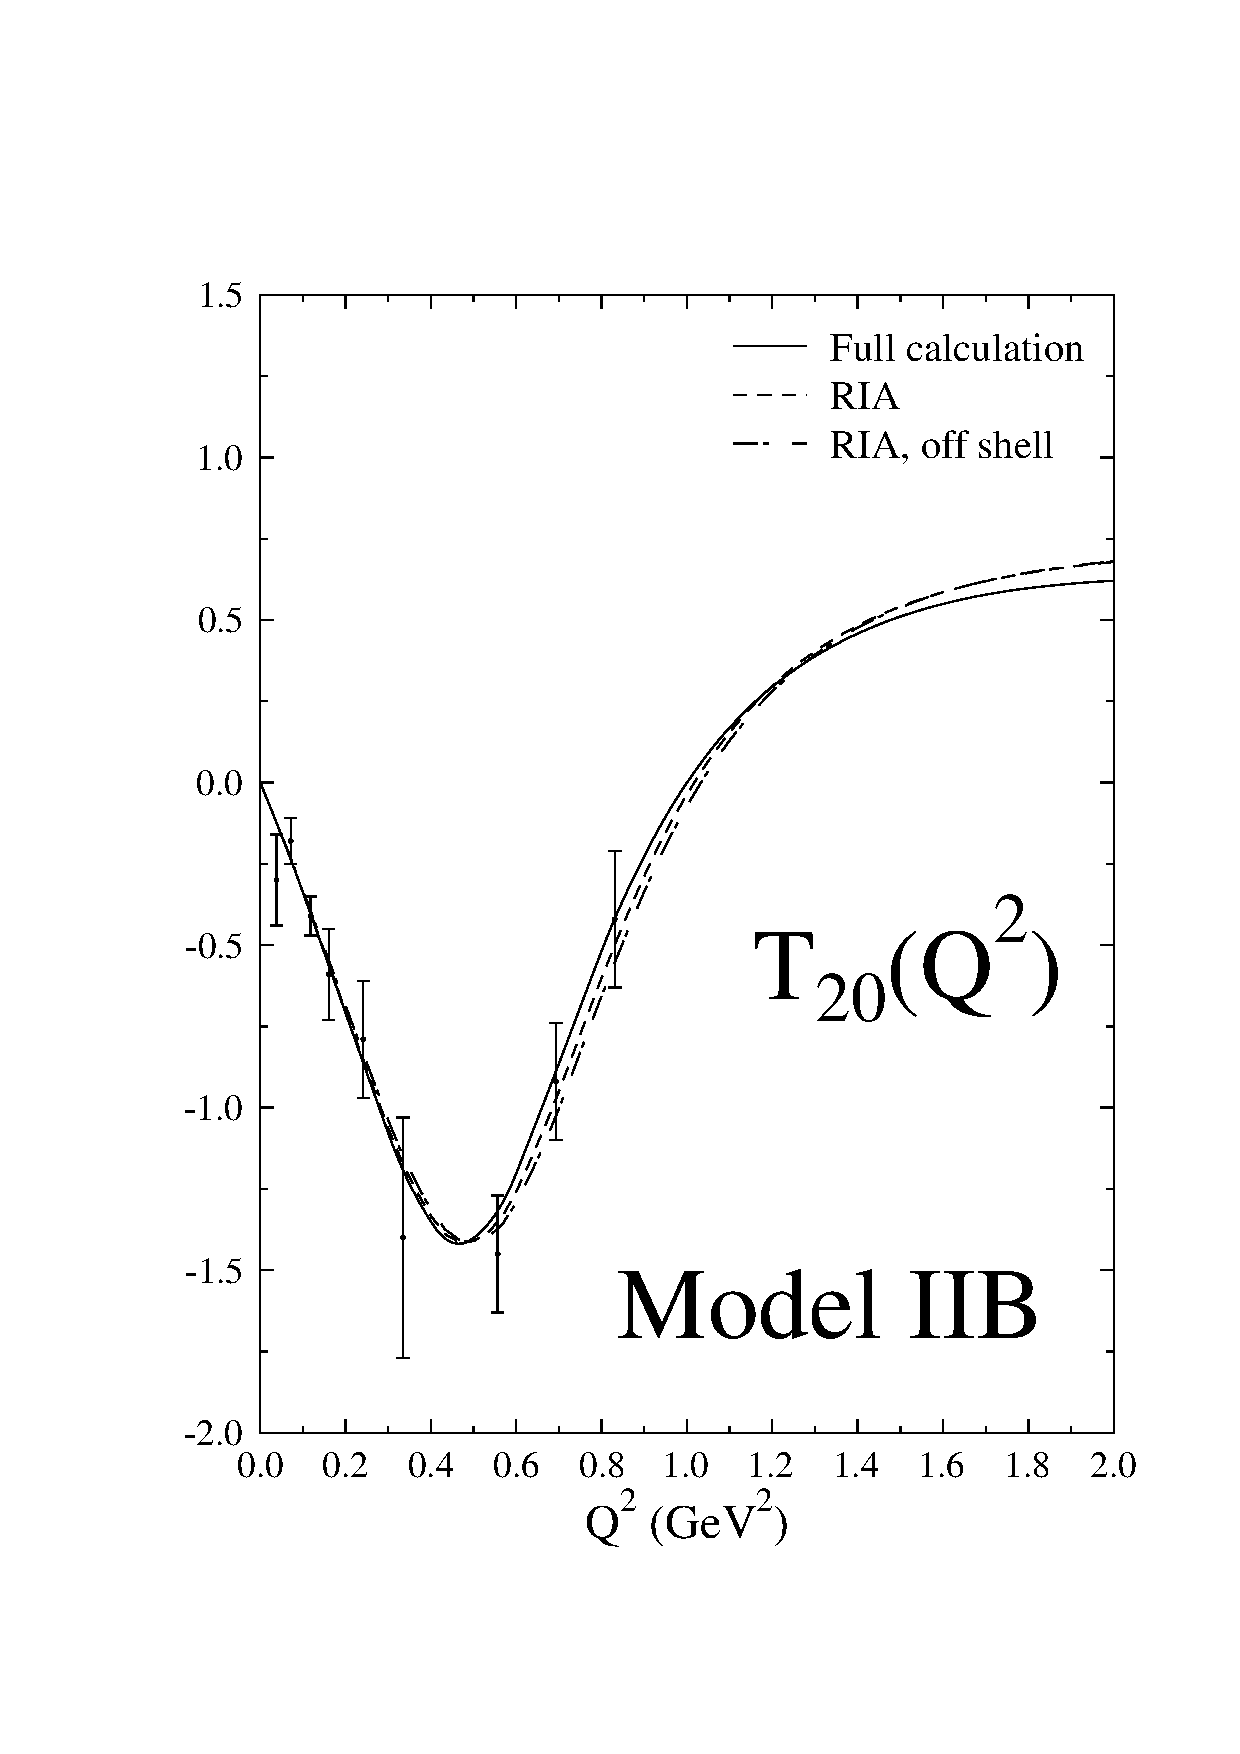
\includegraphics[width=2.75in]{graphics/t20_iib.pdf}}
   \caption{$T_{20}$ for models IB and IIB using the
           spectator equation.}\label{T20}
\end{figure}

Figure \ref{T20} shows $T_{20}(Q^2)$ for models IB and IIB. This function
shows little sensitivity to the various approximations or to the difference
in models. All calculations are in reasonable agreement with the data.

\end{document}
